% Chapter Template

\chapter{Hardware, Technologies and Programming Languages} % Main chapter title

\label{Chapter2} % Change X to a consecutive number; for referencing this chapter elsewhere, use \ref{ChapterX}

\lhead{Chapter 2. \emph{Hardware, Technologies and Programming Languages}} % Change X to a consecutive number; this is for the header on each page - perhaps a shortened title

%----------------------------------------------------------------------------------------
%	SECTION 1
%----------------------------------------------------------------------------------------

\section{Hardware}
Computer hardware (usually simply called hardware when a computing context is implicit) is the collection of physical elements that constitutes a computer system. Computer hardware is the physical parts or components of a computer, such as the monitor, mouse, keyboard, computer data storage, hard disk drive (HDD), system unit (graphic cards, sound cards, memory, motherboard and chips), and so on, all of which are physical objects that can be touched (that is, they are tangible). In contrast, software is instructions that can be stored and run by hardware.


Software is any set of machine-readable instructions that directs a computer's processor to perform specific operations. A combination of hardware and software forms a usable computing system.


%-----------------------------------
%	SUBSECTION 1
%-----------------------------------
\subsection{Raspberry Pi}

\paragraph*{A brief history lesson on the Pi}
\hfill \break
Raspberry Pi \ref{fig:Raspberry} is a series of credit card-sized single-board computers developed in the UK by the Raspberry Pi Foundation with the intention of promoting the teaching of basic computer science in schools.

\begin{wrapfigure}{r}{0.5\textwidth}
  \begin{center}
    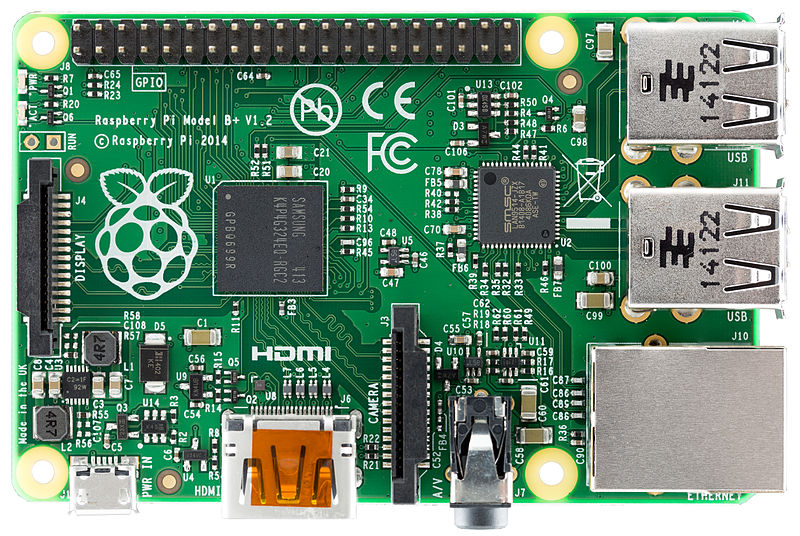
\includegraphics[width=0.5\textwidth]{./Pictures/raspberry_pi_b.jpg}
  \end{center}
  \rule{0.5\textwidth}{0.5pt}
  \caption{Raspberry Pi 1 model B+}
  \label{fig:Raspberry}
\end{wrapfigure}

Over the past decades, computers have gotten cheaper and cheaper, so today
you can find them not only at your desk, but also in nearly every consumer
electronics device, such as smartphones and DVD players. Still, computers
aren’t so cheap that you spontaneously buy one when shopping for your
groceries. Usually, you carefully plan your next computer purchase, because
you have to use it for a couple of years.

Computers like the Raspberry Pi will change the situation completely in the
near future. The Raspberry Pi—or Pi, for short—is a full-blown desktop PC
that costs only \$35. You can connect it directly to the Internet, and it can
display high-definition videos. Also, it runs Linux, so you don’t have to pay
for an operating system. This makes the Pi probably the first throwaway
computer in history.

Originally, the Raspberry Foundation \citep{2} built the Pi to teach children how to
program, so it comes as no surprise that the Pi is an excellent device for
exactly this purpose. On top of that, you can use the Pi for many other
exciting things. For example, you can turn it into a multimedia center, use
it as a cheap but powerful web server, or play some classic games.
The Pi is also a great machine for experimenting with electronics. In contrast
to many popular microcontroller boards, such as the Arduino, the Pi runs a
full-blown operating system, and you can choose from a wide range of programming
languages to implement your projects.
With cheap and small devices like the Raspberry Pi, a new era of ubiquitous
computing has begun, and you can be part of it. This book will help you get
up to speed quickly.

\paragraph*{Get to Know the Hardware}
\hfill \break
Unboxing a new Pi is exciting, but it certainly is not comparable to unboxing
a new Apple product. Usually, the Pi comes in a plain cardboard box with
one or two sheets of paper containing the usual safety hints for electronic
devices and a quick-start guide.


The first version of the Pi looks attractive only to real geeks. It is a singleboard
computer without a case, and it’s the size of a credit card. It somewhat
resembles the innards of the many electronic devices you might have opened
when you were a child.
\subparagraph*{What’s on the Pi}
\hfill \break
The Pi is available in two flavors: Model A and Model B. Model B has been
revised and is available in two slightly different versions now: Model B (Revision
1) and Model B (Revision 2). Model A is a bit cheaper and does not have
as many connectors as Model B. I’ll explain their differences and the differences
between the two Model B revisions in detail in the following text.
I’ll mostly cover Model B in the rest of this book, because it’s much more
popular than Model A. You can see it in Figure \ref{fig:Raspberry_front}

\begin{figure}[h!]
  \centering
    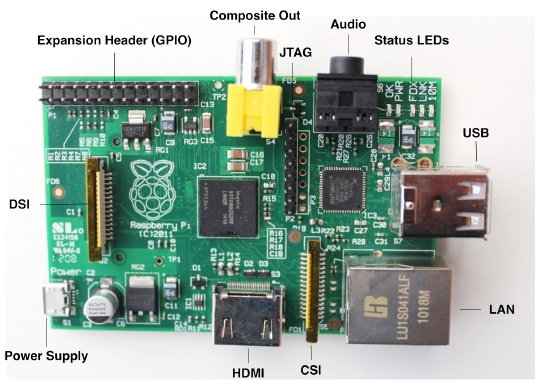
\includegraphics[width=1\textwidth]{./Pictures/raspberry_pi_b_front.jpg}
  \rule{1\textwidth}{0.5pt}
  \caption{The front side of a Model B (Revision 1)}
  \label{fig:Raspberry_front}
\end{figure}

All Raspberry Pi models have the same heart and brain: a system on a chip
(SoC) named BCM2835\cite{3} that you can find in many mobile phones. It’s cheap,
it’s powerful, and it does not consume a lot of power. These characteristics
made it a perfect choice for the Raspberry team.
In contrast to a typical PC architecture, a SoC integrates a processor (CPU),
a graphics processing unit (GPU), and some memory into a single unit. The
BCM2835 contains an ARM1176JZF-S processor running at 700MHz, 512MB
of RAM, and a GPU named VideoCore IV. First-generation devices and Model
A boards have only 256MB of RAM. If you buy a new Pi, make sure it has
512MB of RAM.
For purists, the GPU is a bit problematic because its design and firmware are
proprietary; that is, their source code is not publicly available. This probably
will not affect you in your daily work with the Pi, but it is a problem for some
strong proponents of free software. At least Broadcom has released the source
code for the whole graphics stack under the BSD license.\cite{4} By the time you
read this, the Pi will probably be completely open source.
%-----------------------------------
%	SUBSECTION 2
%-----------------------------------

\subsection{Car Chassis Development Kit}
\begin{figure}[h!]
  \centering
    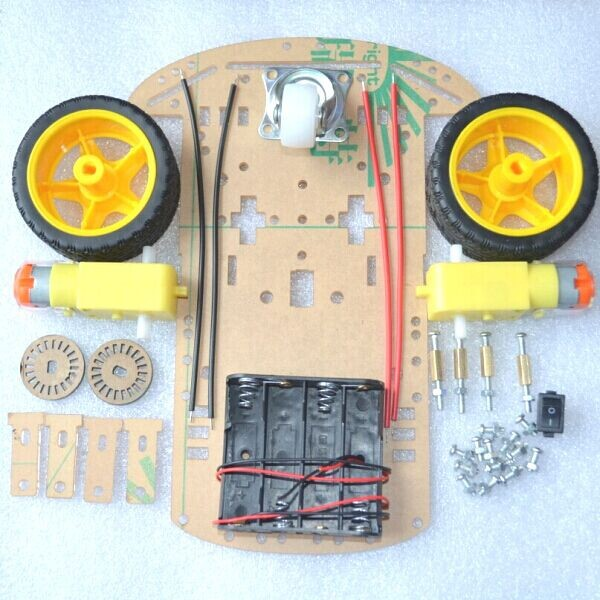
\includegraphics[width=0.5\textwidth]{./Pictures/Car-Chassis-Kit.jpg}
    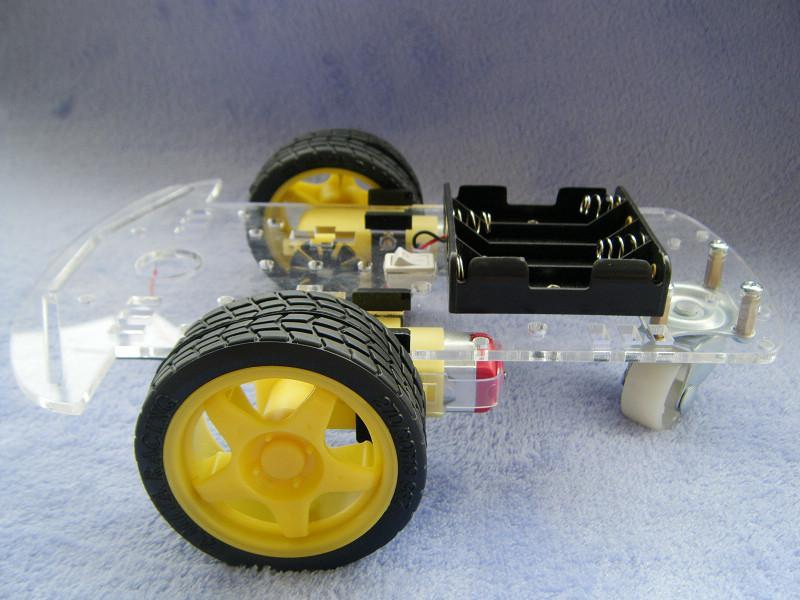
\includegraphics[width=0.5\textwidth]{./Pictures/Car-Chassis-Kit2.jpg}
  \rule{1\textwidth}{0.5pt}
 \caption{Car Chassis Development Kit}
 % \label{fig:Raspberry_front}
\end{figure}
Morbi rutrum odio eget arcu adipiscing sodales. Aenean et purus a est pulvinar pellentesque. Cras in elit neque, quis varius elit. Phasellus fringilla, nibh eu tempus venenatis, dolor elit posuere quam, quis adipiscing urna leo nec orci. Sed nec nulla auctor odio aliquet consequat. Ut nec nulla in ante ullamcorper aliquam at sed dolor. Phasellus fermentum magna in augue gravida cursus. Cras sed pretium lorem. Pellentesque eget ornare odio. Proin accumsan, massa viverra cursus pharetra, ipsum nisi lobortis velit, a malesuada dolor lorem eu neque.


%----------------------------------------------------------------------------------------
%	SECTION 2
%----------------------------------------------------------------------------------------

\section{Technologies and Programming Languages}

Computer software or simply software is any set of machine-readable instructions that directs a computer's processor to perform specific operations. Computer software contrasts with computer hardware, which is the physical component of computers. Computer hardware and software require each other and neither can be realistically used without the other. Using a musical analogy, hardware is like a musical instrument and software is like the notes played on that instrument.
Computer software includes computer programs, libraries and their associated documentation. The word software is also sometimes used in a more narrow sense, meaning application software only.
At the lowest level, executable code consists of machine language instructions specific to an individual processor – typically a central processing unit (CPU). A machine language consists of groups of binary values signifying processor instructions that change the state of the computer from its preceding state. For example, an instruction may change the value stored in a particular storage location inside the computer – an effect that is not directly observable to the user. An instruction may also (indirectly) cause something to appear on a display of the computer system – a state change which should be visible to the user. The processor carries out the instructions in the order they are provided, unless it is instructed to "jump" to a different instruction, or interrupted.
Software written in a machine language is known as "machine code". However, in practice, software is usually written in high-level programming languages that are easier and more efficient for humans to use (closer to natural language) than machine language. High-level languages are translated, using compilation or interpretation or a combination of the two, into machine language. Software may also be written in a low-level assembly language, essentially, a vaguely mnemonic representation of a machine language using a natural language alphabet. Assembly language is translated into machine code using an assembler.


\subsection{Web Application Back-End}
\subsubsection{JavaScript}
JavaScript is the programming language of the Web. The overwhelming majority of
modern websites use JavaScript, and all modern web browsers—on desktops, game
consoles, tablets, and smart phones—include JavaScript interpreters, making JavaScript
the most ubiquitous programming language in history. JavaScript is part of the
triad of technologies that all Web developers must learn: HTML to specify the content
of web pages, CSS to specify the presentation of web pages, and JavaScript to specify
the behavior of web pages. This book will help you master the language.
If you are already familiar with other programming languages, it may help you to know
that JavaScript is a high-level, dynamic, untyped interpreted programming language
that is well-suited to object-oriented and functional programming styles. JavaScript
derives its syntax from Java, its first-class functions from Scheme, and its prototypebased
inheritance from Self. But you do not need to know any of those languages, or
be familiar with those terms, to use this book and learn JavaScript.

The name “JavaScript” is actually somewhat misleading. Except for a superficial syntactic
resemblance, JavaScript is completely different from the Java programming language.
And JavaScript has long since outgrown its scripting-language roots to become
a robust and efficient general-purpose language. The latest version of the language (see
the sidebar) defines new features for serious large-scale software development.

\paragraph*{JavaScript: Names and Versions}
\hfill \break
JavaScript was created at Netscape in the early days of the Web, and technically, “JavaScript”
is a trademark licensed from Sun Microsystems (now Oracle) used to describe
Netscape’s (now Mozilla’s) implementation of the language. Netscape submitted the
language for standardization to ECMA—the European Computer Manufacturer’s Association—and
because of trademark issues, the standardized version of the language
was stuck with the awkward name “ECMAScript.” For the same trademark reasons,
Microsoft’s version of the language is formally known as “JScript.” In practice, just
about everyone calls the language JavaScript. This book uses the name “ECMAScript”
only to refer to the language standard.


For the last decade, all web browsers have implemented version 3 of the ECMAScript
standard and there has really been no need to think about version numbers: the language
standard was stable and browser implementations of the language were, for the
most part, interoperable. Recently, an important new version of the language has been
defined as ECMAScript version 5 and, at the time of this writing, browsers are beginning
to implement it. This book covers all the new features of ECMAScript 5 as well as all
the long-standing features of ECMAScript 3. You’ll sometimes see these language versions
abbreviated as ES3 and ES5, just as you’ll sometimes see the name JavaScript
abbreviated as JS.


When we’re speaking of the language itself, the only version numbers that are relevant
are ECMAScript versions 3 or 5. (Version 4 of ECMAScript was under development
for years, but proved to be too ambitious and was never released.) Sometimes, however,
you’ll also see a JavaScript version number, such as JavaScript 1.5 or JavaScript 1.8.
These are Mozilla’s version numbers: version 1.5 is basically ECMAScript 3, and later
versions include nonstandard language extensions. Finally, there are
also version numbers attached to particular JavaScript interpreters or “engines.” Google
calls its JavaScript interpreter V8, for example, and at the time of this writing the
current version of the V8 engine is 3.0.


\paragraph*{Exploring JavaScript}
\hfill \break
When learning a new programming language, it’s important to try the examples in the
book, and then modify them and try them again to test your understanding of the
language. To do that, you need a JavaScript interpreter. Fortunately, every web browser
includes a JavaScript interpreter, and if you’re reading this book, you probably already
have more than one web browser installed on your computer.

We’ll see later on in this chapter that you can embed JavaScript code within <script>
tags in HTML files, and when the browser loads the file, it will execute the code. Fortunately,
however, you don’t have to do that every time you want to try out simple
snippets of JavaScript code. Spurred on by the powerful and innovative Firebug extension
for Firefox (pictured in Figure \ref{fig:Firebug} and available for download from \href{http://getfirebug.com/}{http://getfirebug.com/}, today’s web browsers all include web developer tools that are indispensable for
debugging, experimenting, and learning. You can usually find these tools in the Tools
menu of the browser under names like “Developer Tools” or “Web Console.”
(Firefox 4 includes a built-in “Web Console,” but at the time of this writing, the Firebug
extension is better.) Often, you can call up a console with a keystroke like F12 or Ctrl-Shift-J.
These console tools often appear as panes at the top or bottom of the browser
window, but some allow you to open them as separate windows (as pictured in Figure
\ref{fig:Firebug}), which is often quite convenient.


A typical “developer tools” pane or window includes multiple tabs that allow you to
inspect things like HTML document structure, CSS styles, network requests, and so
on. One of the tabs is a “JavaScript console” that allows you to type in lines of JavaScript
code and try them out. This is a particularly easy way to play around with JavaScript,
and I recommend that you use it as you read this book.

There is a simple console API that is portably implemented by modern browsers. You
can use the function console.log() to display text on the console. This is often surprisingly
helpful while debugging, and some of the examples in this book (even in the
core language section) use console.log() to perform simple output. A similar but more
intrusive way to display output or debugging messages is by passing a string of text to
the alert() function, which displays it in a modal dialog box.
\begin{figure}[h!]
  \centering
    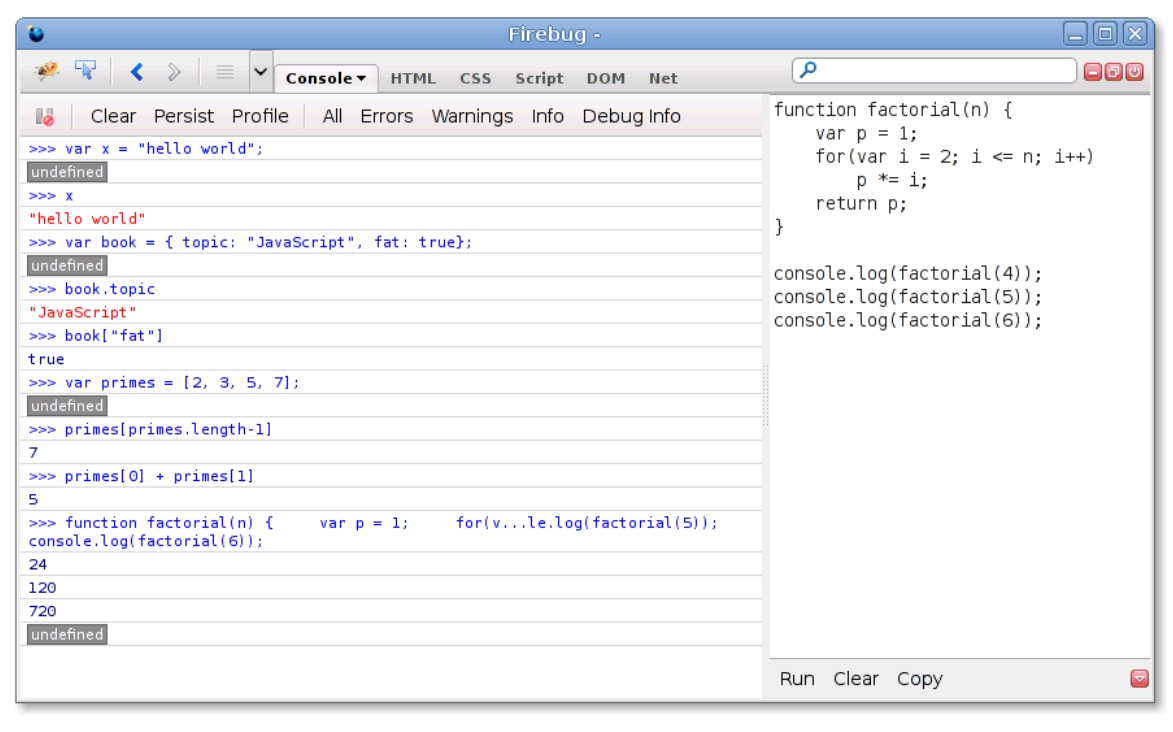
\includegraphics[width=\textwidth]{./Pictures/firebug.jpg}
  \rule{1\textwidth}{1pt}
 \caption{The Firebug debugging console for Firefox}
 \label{fig:Firebug}
\end{figure}


\subsubsection{NodeJs}
Node.js is an open source, cross-platform runtime environment for server-side and networking applications. Node.js applications are written in JavaScript, and can be run within the Node.js runtime on OS X, Microsoft Windows, Linux, FreeBSD, NonStop and IBM i.

Node.js provides an event-driven architecture and a non-blocking I/O API that optimizes an application's throughput and scalability. These technologies are commonly used for real-time web applications.
Node.js uses the Google V8 JavaScript engine to execute code, and a large percentage of the basic modules are written in JavaScript. Node.js contains a built-in library to allow applications to act as a Web server without software such as Apache HTTP Server or IIS.
\paragraph*{History}
\hfill \break
Node.js was invented in 2009 by Ryan Dahl, and other developers working at Joyent. Node.js was created and first published for Linux use in 2009. Its development and maintenance was spearheaded by Ryan Dahl and sponsored by Joyent, the firm where Dahl worked.

Dahl was inspired to create Node.js after seeing a file upload progress bar on Flickr. The browser did not know how much of the file had been uploaded and had to query the Web server. Dahl desired an easier way.

It garnered international attention after its debut at the inaugural European JSConf on November 8, 2009. Dahl presented Node.js, which combined Google's V8 JavaScript engine, an event-loop, and a low-level I/O API. The project received a standing ovation, and has since then experienced significant growth, popularity and adoption.

In 2011, a package manager was introduced for Node.js library, called npm. The package manager allows publishing and sharing of open-source Node.js libraries by the community, and simplifies installation, updating and uninstallation of libraries.

In June 2011, Microsoft partnered with Joyent to implement a native Windows version of Node.js. The first Node.js build to support Windows was released in July.

In January 2012, Dahl stepped aside, promoting coworker and npm creator Isaac Schlueter to manage the project.

In January 2014, Schlueter announced Timothy J. Fontaine would be Node.js's new project lead.

In December 2014, Fedor Indutny started io.js, a fork of Node.js. Due to internal conflict over Joyent's governance, io.js was created as an open governance alternative with a separate technical committee.

\subsubsection{ExpressJs}
Express.js is a Node.js web application framework, designed for building single-page, multi-page, and hybrid web applications.
Express is a minimal and flexible Node.js web application framework that provides a robust set of features for web and mobile applications.
\subsubsection{Socket.io}
Socket.IO enables real-time bidirectional event-based communication.
It works on every platform, browser or device, focusing equally on reliability and speed.
\subsection{Web Application Front-End} 
\subsubsection{HTML (HyperText Markup Language)}
\subsubsection{CSS (Cascading Style Sheets)}
\subsubsection{Less}
\subsubsection{CoffeeScript}
\subsubsection{jQuery}
\subsection{Tools Used for Developing}
\subsubsection{Sublime Text 3}
\subsubsection{GruntJs}
\subsubsection{PuTTY}
\subsubsection{Basic UNIX commands }
